\section{Die starke Markoveigenschaft}

Bis jetzt haben wir gesehen, dass $(W_{s+t} - W_s)_{t \geq 0}$ ein Wiener-Prozess ist, der von $\sF := \sigma(W_r : r \leq s)$ unabh�ngig ist. Wir wollen dies nun auf Stoppzeiten verallgemeinern.

\begin{definition}[Stoppzeit]\label{Nummer5.3.1}
Sei $\sF = (\sF_t)_{t \geq 0}$ eine Filtration und $\tau\colon \Omega \to [0, \infty]$. Dann hei�t $\tau$ \deftxt{$\sF$-Stoppzeit}\index{Stoppzeit} genau dann, wenn $\{\tau \leq t\} \in \sF_t$ f�r alle $t \geq 0$ gilt.
\end{definition}

\begin{beispiel}[Passierzeit von Wiener-Prozessen]\label{Nummer5.3.2}
F�r $a \in \R$ ist $\tau_a := \inf\{t \geq 0 : W_t = a\}$ eine Stoppzeit. Den Beweis, der die Stetigkeit der Pfade verwendet, �berlassen wir zur �bung.
\end{beispiel}

Analog zu Definition \ref{Nummer5.3.1} wollen wir auch andere bereits aus fr�heren Kapiteln bekannte Begriffe definieren:
\begin{itemize}
	\item Der Prozess $(X_t)$ hei�t an die Filtration $\sF = (\sF_t)_{t \geq 0}$ \deftxt{adaptiert}\index{Stochastischer Prozess!adaptierter}, falls $\{X_t \in B\} \in \sF_t$ f�r alle $t \geq 0$ und $B \in \sB$ gilt.
	\item Sei $\tau$ eine endliche $\sF$-Stoppzeit und $(X_t)$ ein an $\sF$ adaptierter Prozess. Dann setzen wir $X_\tau\colon \Omega \to \R$ mit $X_\tau(\omega) := X_{\tau(\omega)}(\omega)$ f�r $\omega \in \Omega$.
	\item Die \deftxt{$\sigma$-Algebra der $\tau$-Vergangenheit}\index{$\tau$-Vergangenheit} ist definiert durch
	\begin{align*}
	\sF_\tau &:= \{A \in \sA : A \cap \{\tau \leq t\} \in \sF_t \quad \forall_{t \geq 0}\}\text{.}
	\end{align*}
\end{itemize}
Im zeitdiskreten Fall ist $X_\tau$ auch $\sF_\tau$-messbar. Im zeitkontinuierlichen Fall gilt dies im Allgemeinen jedoch nicht. Dies f�hrt zu folgender Definition:

\begin{definition}[Progressiv-Messbarkeit]\label{Nummer5.3.3}
Ein stochastischer Prozess $X = (X_t)_{t \geq 0}$ hei�t \deftxt{$\sF$-progressiv-messbar}\index{Messbarkeit!Progressiv-} genau dann, wenn die Abbildung
\begin{align*}
\Omega \times [0, t] &\to \R\text{,}\\
(\omega, s) &\mapsto X_s(\omega)
\end{align*}
$\sF_t \otimes \B([0,t])$-messbar f�r alle $t \geq 0$ ist.
\end{definition}
Mit anderen Worten fordert man also gemeinsame Messbarkeit in $\omega$ und $s$. Ist $(X_t)$ $\sF$-progressiv-messbar, so ist $(X_t)$ insbesondere $\sF$-adaptiert. 

\begin{lemma}\label{Nummer5.3.4}
Ist $(X_t)$ $\sF$-adaptiert und links- oder rechtsstetig, so ist $(X_t)$ auch progressiv-messbar. Insbesondere sind Wiener-Prozesse, homogene Poissonprozesse und inhomogene Poissonprozesse progressiv-messbar.
\end{lemma}

\begin{beweis}
Wir behandeln hier nur den rechtsstetigen Fall und nehmen ohne Einschr�nkung $t = 1$ an. Definiere nun
\begin{align*}
Y_n(\omega, s) &:= \begin{cases} X_{(j+1)2^{-n}}(\omega) & \text{f�r } s \in [j2^{-n}, (j+1)2^{-n})\text{, } j = 0, \ldots, 2^n - 1\\ X_s(\omega) & \text{f�r } s \geq 1\end{cases}\text{.}
\end{align*}
Da $(X_t)$ rechtsstetig ist, folgt $\lim_{n \to \infty} Y_n(\omega, s) = X_s(\omega)$ f�r $(\omega, s) \in \Omega \times [0, \infty)$. Wir zeigen noch, dass $Y_n\big|_{\Omega \times [0,t]}$ messbar bez�glich $\sF_1 \otimes \sB([0,1])$ ist. Dazu betrachten wir
\begin{align*}
\{Y_n \in B\} &= \bigcup_{j=0}^{2^n - 1} \{ X_{(j+1)2^{-n}} \in B\} \times [j2^{-n}, (j+1)2^{-n}) \cup \{X_1 \in B\} \times \{1\}\\
\quad &\in \sF_1 \otimes \sB([0,1])\text{.} \qedhere
\end{align*}
\end{beweis}

\begin{satz}[Messbarkeit von $X_\tau$]\label{Nummer5.3.5}
Sei $\sF = (\sF_t)$ eine Filtration, $X = (X_t)$ sei ein $\sF$-progressiv-messbarer stochastischer Prozess und $\tau$ eine $\sF$-Stoppzeit. Dann ist $X_\tau$ $\sF_\tau$-messbar.
\end{satz}

\begin{beweis}
Sei $B \subset \sB$ und $t \geq 0$. Wir wollen zeigen, dass $\{X_\tau \in B\} \cap \{\tau \leq t\} \in \sF_t$ gilt, diese Menge ist aber darstellbar als $\{X_{\tau \wedge t} \in B\} \cap \{\tau \leq t\}$ und es gilt $\{\tau \leq t\} \in \sF_t$, es gen�gt also $\{X_{\tau \wedge t} \in B\} \in \sF_t$ zu zeigen. Da $\tau \wedge t \leq t$ eine Stopzeit ist, k�nnen wir ohne Einschr�nkung annehmen, dass $\tau \leq t$ gilt, zeigen also $\{X_\tau \in B\} \in \sF_t$, also die $\sF_t$-Messbarkeit von $X_\tau$. Dazu betrachten wir $\psi\colon \Omega \to \Omega \times [0,t]$ mit $\omega \mapsto (\omega, \tau(\omega))$. F�r $A \in \sF_t$ und $u \leq t$ gilt nun
\begin{align*}
\{\psi \in A \times [0, u]\} &= \{\omega \in \Omega : \omega \in A \text{ und } \tau(\omega) \leq u\} = A \cap \underbrace{\{\tau \leq u\}}_{\in \sF_u \subset \sF_t} \in \sF_t\text{,}
\end{align*}
also ist $\psi$ messbar bez�glich $(\sF_t, \sF_t \otimes \sB([0, t]))$. Ferner gilt $X_\tau = X \circ \psi$ und da $X$ bez�glich $(\sF_t \otimes \sB([0,t]), \sB)$ messbar ist folgt daher, dass $X_\tau$ als Komposition $(\sF_t, \sB)$-messbar ist.
\end{beweis}

\begin{satz}[Starke Markoveigenschaft des Wiener-Prozesses]\label{Nummer5.3.6}
Es sei $(W_t)_{t \geq 0}$ ein Wiener-Prozess mit nat�rlicher Filtration $\sF = (\sF_t)$ und $\tau\colon \Omega \to [0, \infty]$ eine fast sicher endliche $\sF$-Stoppzeit. Dann ist $(X_t)_{t \geq 0}$ definiert durch $X_t := W_{t + \tau} - W_\tau$ f�r $t \geq 0$ ein Wiener-Prozess, der von $\sF_\tau$ unabh�ngig ist.
\end{satz}

Ist $\tau = t_0$ konstant, so entspricht dies der einfachen Markoveigenschaft aus Korollar \ref{Nummer5.1.9}.

\begin{beweis}
Wir wollen folgende Identit�ten f�r alle $t_1 < \ldots < t_n$, $n \geq 1$, $A \in \sB^n$ und $B \in \sF_\tau$ zeigen:
\begin{center}
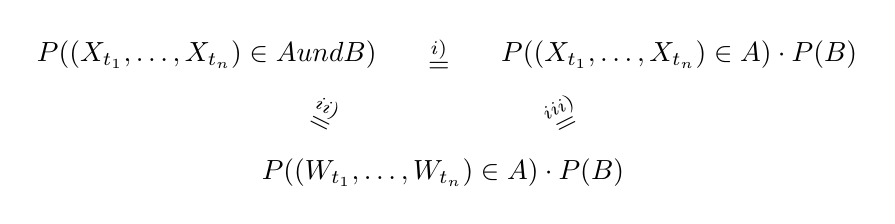
\begin{tikzpicture}
\node (A) at (0, 0) {$\displaystyle P((X_{t_1}, \ldots, X_{t_n}) \in A \text{ und } B)$};
\node (B) at (6, 0) {$\displaystyle P((X_{t_1}, \ldots, X_{t_n}) \in A) \cdot P(B)$};
\node (C) at (3, -1.5) {$\displaystyle P((W_{t_1}, \ldots, W_{t_n}) \in A) \cdot P(B)$};

\path (A) -- node[sloped] {$\stackrel{\text{i)}}{=}$} (B);
\path (A) -- node[sloped] {$\stackrel{\text{ii)}}{=}$} (C);
\path (B) -- node[sloped] {$\stackrel{\text{iii)}}{=}$} (C);
\end{tikzpicture}
\end{center}
Ist dies gezeigt, so folgt die Unabh�ngigkeit aus i) und da $(W_t)$ und $(X_t)$ nach iii) die selben Randverteilungen besitzen, ist $(X_t)$ ein zentrierter Gau�-Prozess mit Kovarianzfunktion $\Gamma(s,t) = \min\{s, t\}$. Da $(X_t)$ offensichtlich auch stetig ist, folgt nach Satz \ref{Nummer5.1.6} also, dass $(X_t)$ ein Wiener-Prozess ist. Der Beweis von i) -- iii) erfolgt nun in zwei Schritten:

Im ersten Schritt nehmen wir an, dass $\tau$ nur abz�hlbar viele Werte annimmt. Sei $\tau(\Omega)$ also abz�hlbar und $(s_n)_{n \geq 1}$ eine entsprechende Abz�hlung. F�r $n \geq 1$ und $B \in \sF_\tau$ gilt dann
\begin{align*}
B \cap \{\tau = s_n\} &= \underbrace{B \cap \{\tau \leq s_n\}}_{\in \sF_{s_n}} \cap \{\tau = s_n\}\text{,}
\end{align*}
der letzte Teil l�sst sich als $\{\tau = s_n\} = \{\tau \leq s_n\} \setminus \bigcup_{s_m < s_n} \{\tau \leq s_m\}$ schreiben l�sst. Nun ist $\{\tau \leq s_n\} \in \sF_{s_n}$ und $\{\tau \leq s_m\} \in \sF_{s_m} \subset \sF_{s_n}$, insgesamt also $B \cap \{\tau = s_n\} \in \sF_{s_n}$. Auf $\{\tau = s_n\}$ gilt nun $X_t = W_{t + \tau} - W_\tau = W_{t + s_n} - W_{s_n} =: Y_t^{(n)}$. Beachte, dass $(Y^{(n)})_{t \geq 0}$ ein Wiener-Prozess ist, der nach Korollar \ref{Nummer5.1.9} von $\sF_{s_n}$ unabh�ngig ist. Nun folgt
\begin{align*}
P((X_{t_1}, \ldots, X_{t_n}) \in A \text{ und } B) &= \sum_{n=1}^\infty P((X_{t_1}, \ldots, X_{t_n}) \in A \text{ und } B \cap \{\tau = s_n\})\\
\quad &= \sum_{n=1}^\infty P((Y_{t_1}^{(n)}, \ldots, Y_{t_n}^{(n)}) \in A \text{ und } B \cap \{\tau = s_n\})\\
\quad &= \sum_{n=1}^\infty P((Y_{t_1}^{(n)}, \ldots, Y_{t_n}^{(n)}) \in A)P(B \cap \{\tau = s_n\})\\
\quad &= \sum_{n=1}^\infty P((W_{t_1}, \ldots, W_{t_n}) \in A)P(B \cap \{\tau = s_n\})\\
\quad &= P((W_{t_1}, \ldots, W_{t_n}) \in A)P(B)\text{.}
\end{align*}
Damit ist iii) gezeigt. Setzt man $B := \Omega$, so folgt auch ii).

Im zweiten Schritt sei $\tau$ allgemein. F�r $n \in \N_0$ sei $\tau_n := \sum_{k=0}^\infty \frac{k+1}{2^n}\ind_{\{k2^{-n} \leq \tau < (k+1)2^{-n}\}}$ und $\tau_n(\omega) := \infty$, falls $\tau(\omega) = \infty$ ist. Offensichtlich ist $\tau_n(\Omega)$ abz�hlbar. Zu zeigen ist also, dass $\tau_n$ eine Stoppzeit ist. F�r $0 \leq t < 2^{-n}$ gilt $\{\tau_n \leq t\} = \emptyset \in \sF_t$. F�r $2^{-n} \leq t$ gibt es ein $k_0 \geq 0$ mit $(k_0+1)2^{-n} \leq t < (k_0+2)2^{-n}$. Dann folgt
\begin{align*}
\{\tau_n \leq t\} &= \bigcup_{k=0}^{k_0} \left\{\tau_n = \frac{k+1}{2^n}\right\} = \bigcup_{k=0}^{k_0} \underbrace{\left\{k2^{-n} \leq \tau < (k+1)2^{-n}\right\}}_{\in \sF_{(k+1)2^{-n}}}\\
\quad &\in \sF_{(k_0 + 1)2^{-n}} \subset \sF_t\text{.}
\end{align*}
Ferner ist $\tau_n \geq \tau$ und $\tau_n \searrow \tau$. F�r $n \in \N_0$ setzen wir nun $Y_t^{(n)} := W_{t + \tau_n} - W_{\tau_n}$, dann ist $Y_t^{(n)}$ gem�� dem ersten Schritt ein Wiener-Prozess. Da Wiener-Prozesse stetig sind, folgt $Y_t^{(n)} \stackrel{n \to \infty}{\longrightarrow} X_t$ $P$-fast sicher. Ferner sei $B \in \sF_\tau \subset \sF_{\tau_n}$, mit dem ersten Schritt folgt dann $P((Y_{t_1}^{(n)}, \ldots, Y_{t_m}^{(n)}) \in A \text{ und } B) = P((W_{t_1}, \ldots, W_{t_m}) \in A)P(B)$. Da $P$-fast sichere Konvergenz die Konvergenz in Verteilung impliziert, folgt insgesamt
\begin{align*}
P((X_{t_1}, \ldots, X_{t_m}) \in A)P(B) &= P((W_{t_1}, \ldots, W_{t_m}) \in A)P(B)\text{.}
\end{align*}
Damit ist wieder iii) gezeigt und ii) folgt wiederum mit $B = \Omega$.
\end{beweis}